\documentclass[a4]{article}

\usepackage[icelandic]{babel}
\usepackage[T1]{fontenc}
\usepackage{amsmath}
\usepackage{graphicx}
\usepackage{sidecap}
\usepackage[utf8]{inputenc}
\usepackage[left=1in,top=1in,right=1in,bottom=1in,nohead]{geometry}
\usepackage[framed,numbered,autolinebreaks,useliterate]{mcode}
\usepackage{epstopdf}
\title{Töluleg Greining\\ Verkefni 7}
\date{\today{}}
\author{ 
  Bjarki Geir Benediktsson,\and
  Haukur Óskar Þorgeirsson,\and
  Matthías Páll Gissurarson \and
  Kennari: Máni Maríus Viðarsson
  }
\begin{document}
\maketitle
\section{Dæmi 7}

Við notuðum það sem gefið var og fengum út eftirfarandi
mismunakvótatöflu.
$$
  \begin{array}{|l|l|l|l|l|l|l|}
    \hline
    i & x_i & f[x_i] & f[x_i,x_{i+1}] & f[x_i,x_{i+1},x_{i+2}] & f[x_i,x_{i+1},x_{i+2},x_{i+3}] & f[x_i,x_{i+1},x_{i+2},x_{i+3},x_i{+4}] \\
    \hline
    0 & -1 & 0.5 & 0 & 0.5 & -0.3125 & 0.125 \\
    1 & -1 & 0.5 & 0.5 & -0.125 & -0.0625 & \\
    2 & 0 & 1 & 0.25 & -0.25 & & \\
    3 & 1 & 1.25 & 0 & & & \\
    4 & 1 & 1.25 & & & &
  \end{array}
$$

en út frá henni fæst að

$$p(x) = 0.5 + 0.5(x+1)^2 - (5/16)(x+1)^2x + (1/8)(x+1)^2x(x-1)$$\\
$$= \frac{x^4}{8}-\frac{3x^3}{16}-0.25 x^2+ 0.5625 x+1,$$

og $$p(0.3) = 0.5 + 0.5\cdot 1.3^2 - (5/16)(1.3^2)\cdot 0.3 + 0.125
\cdot 1.3^2\cdot 0.3 \cdot -0.7 = 1.1422.$$

Við fáum svo út frá ójöfnunni $-1 \leq f^{(5)}(x) \leq 4$ að
$$-0.00207025 = -1 \cdot \frac{(0.3+1)^2\cdot 0.3 \cdot (0.3-1)^2}{5!}
\leq f(0.3) - p(0.3) \leq 4 \cdot \frac{(0.3+1)^2\cdot 0.3 \cdot
  (0.3-1)^2}{5!} = 0.008281,$$ svo
$$1.14012975 \leq f(0.3) \leq 1.150481$$ en lengd bilsin er $|0.008281 + 0.00207025| = 0.01035125$.  Ef við notum miðpunkt bilsins til að nálga
$f(0.3)$ og rúnum af miðað við leng bilsins fáum við fáum við þá
$f(0.3) = 1.14012975 + 0.005175625 = 1.145305374 \pm 0.005175625 = 1.15 \pm 0.01$.

\section{Dæmi 8}

\subsection{a)}

Við höfum mæligildin:

\begin{center}
	\begin{tabular}{c|l|l|l|l|l}
	  x&0.0&0.4&0.7&0.9&1.0\\ \hline
		y&1.22&0.53&0.34&0.72&1.22\\
	\end{tabular}
\end{center}

Við höfum, líkt og í glærunum, $s_i$, einskorðun $s$ við hvert bil $[t_i,t_{i+1}]$ ($t_i$ verandi x gildin að ofan, $i = 0,..,4$) þar sem $s_i(x) = a_i + b_i(x-t_i) + c_i(x-t_i)^2 + d_i(x-t_i)^3$. Við vitum að $a_i = y_i,\, i = 0,..,4$. Þannig eru\\
$$
\begin{array}{rcl}
	s_0(x)&=&1.22 + b_0(x-0.0) + c_0(x-0.0)^2 + d_0(x-0.0)^3 = a_0 + b_0x + c_0x^2 + d_0x^3\\
	s_1(x)&=&0.53 + b_1(x-0.4) + c_1(x-0.4)^2 + d_1(x-0.4)^3\\
	s_2(x)&=&0.34 + b_2(x-0.7) + c_2(x-0.7)^2 + d_2(x-0.7)^3\\
	s_3(x)&=&0.72 + b_3(x-0.9) + c_3(x-0.9)^2 + d_3(x-0.9)^3
\end{array}\\
$$
Út frá reglunum sem skilgreina splæsibrúun með lotubundna splæsibrúun fæst því
$$
\begin{bmatrix}
1&0&0&0&-1\\
0.4&2(0.4+0.3)&0.3&0&0\\
0&0.3&2(0.3+0.2)&0.2&0\\
0&0&0.2&2(0.2+0.1)&0.1\\
0&0.4&0&2(0.1)&2(0.4+0.1)
\end{bmatrix}
\begin{bmatrix}
c_0\\
c_1\\
c_2\\
c_3\\
c_4
\end{bmatrix}
=
\begin{bmatrix}
1&0&0&0&-1\\
0.4&1.4&0.3&0&0\\
0&0.3&1.0&0.2&0\\
0&0&0.2&0.6&0.1\\
0&0.4&0&0.2&1.0
\end{bmatrix}
\begin{bmatrix}
c_0\\
c_1\\
c_2\\
c_3\\
c_4
\end{bmatrix}
=3
\begin{bmatrix}
  0\\
	\frac{0.34-0.53}{0.3} - \frac{0.53-1.22}{0.4}\\
	\frac{0.72-0.34}{0.2} - \frac{0.34-0.53}{0.3}\\
	\frac{1.22-0.72}{0.1} - \frac{0.72-0.34}{0.2}\\
	\frac{0.53-1.22}{0.4} - \frac{1.22-0.72}{0.1}
	
\end{bmatrix}\\
$$
Gott er að muna að efsta og neðsta línan í hverju fylki nema $c_i$ fylkinu eru fengnar úr því að við notum lotubundin endaskilyrði.

Við vitum $a_i$, og höfum nú fundið $c_i$ með því að leysa þetta jöfnuhneppi($i=0,..,4$). Þá getum við leyst $b_i$ og $d_i$ ($i=0,..,3$) út úr eftirfarandi jöfnum, sem sjálfar koma úr skilgreiningu á splæsibrúun: ($h_i=t_{i+1} - t_i$)\\

$\begin{array}{rcrl}
	a_i + b_ih_i + c_ih_i^2 + d_ih_i^3&=&a_{i+1},&i=0,..,3\\
	b_i + 2c_ih_i + 3d_ih_i^2&=&b_{i+1},&i=0,..,3\\
	2c_i + 6d_ih_i&=&2c_{i+1},&i=0,..,3
\end{array}$

Þegar búið er að reikna $a_2, \, b_2, \, c_2,$ og $d_2$ höfum við fundið $s_2(x) = s(x)\{ {[0.7,0.9]}\}$, en þá getum við nálgað $f(0.8)$ með því að reikna $s(0.8)=s_2(0.8)$.
\subsection{b}
\begin{align*}
\begin{bmatrix}
1&0		&0	\\
1&0.4-0.4^2	&e^{0.4}\\
1&0.7-0.7^2	&e^{0.7}\\
1&0.9-0.9^2	&e^{0.9}\\
1&0		&1
\end{bmatrix}
=
\begin{bmatrix}
1&0    &1     \\
1&0.24&1.49182\\
1&0.21&2.01375\\
1&0.09&2.45960\\
1&0   &2.71828
\end{bmatrix}
\end{align*}
Fáum að jafnan fyrir fallið er
$$ 1.342718-3.4114457\cdot x(1-x)-0.086891\cdot e^x$$
\lstinputlisting{v5.m}

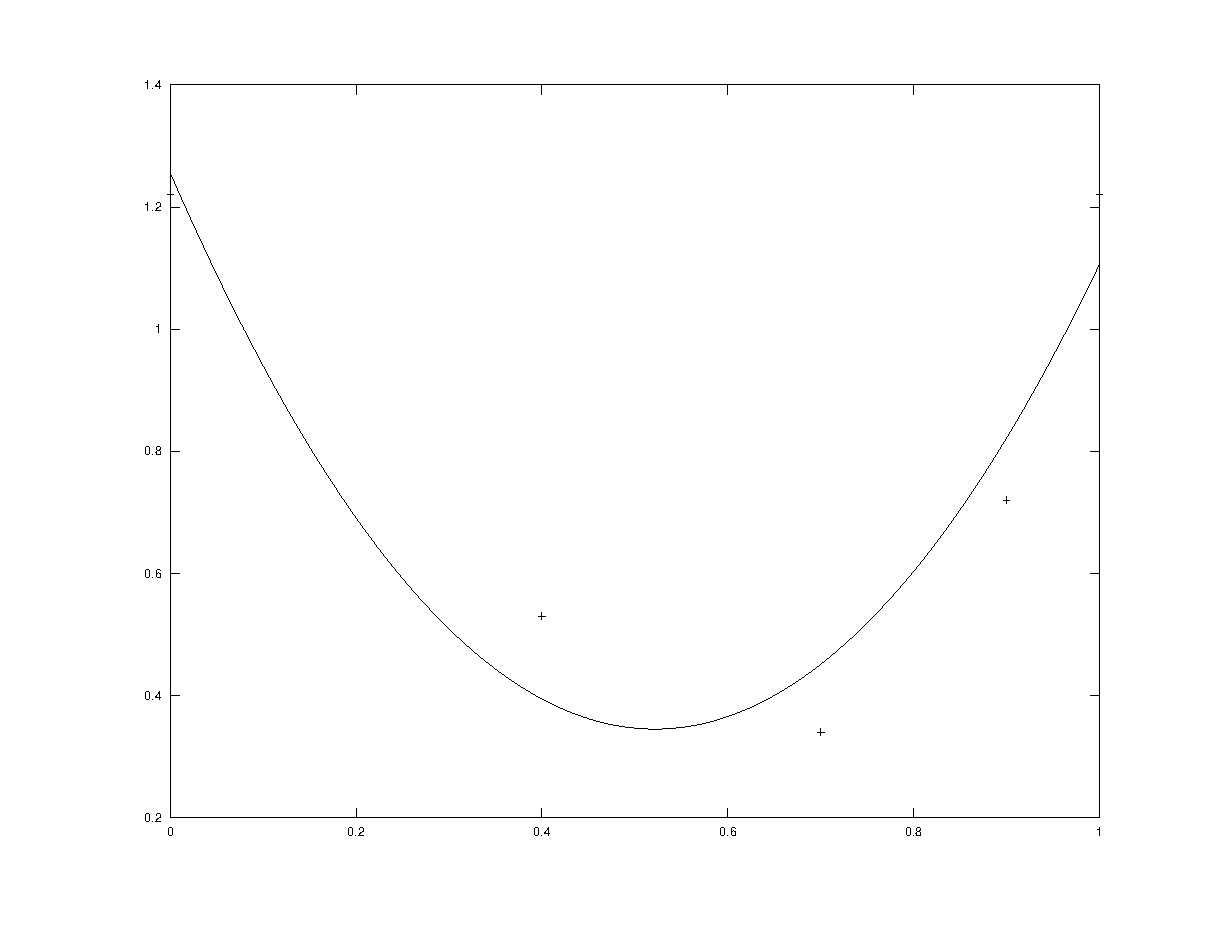
\includegraphics[width=14cm]{d5.eps}
\end{document}
